\section{Overview}
\label{sec:background}

\begin{figure*}
\begin{subfigure}{.6\textwidth}
\begin{func}[$\Func_{\textsc{com}}$]
    $\Func_{\textsc{com}}$ proceeds as follows, running with parties $A$ and
  $B$.
    \begin{enumerate}
        \item Upon receiving a message $(\mathsf{Commit}, b)$ from $A$, where $b
          \in \{ 0, 1 \}$, record the value $b$ and send the message
          $(\mathsf{Receipt})$ to $B$. Ignore any subsequent \textsf{Commit}
          messages.
        \item Upon receiving a message $(\mathsf{Open})$ from $A$, proceed as
          follows: If some value $b$ was previously recorded, then send the
          message $(\mathsf{Open}, b)$ to $B$ and halt. Otherwise, halt.
    \end{enumerate}
\end{func}
%\caption{An ideal functionality for a one-time commitment scheme.}
\label{func:com}
\end{subfigure}\hspace{.04\textwidth}%
\begin{subfigure}{.35\textwidth}
  \lstinputlisting[style=myilc]{listings/Fcom.ilc}
\end{subfigure}
\caption{An ideal functionality for a one-time commitment scheme in prose (left)
  and in ILC (right).}
\label{func:com}
\end{figure*}

\subsection{Ideal Functionalities}
\label{subsec:functionalities}

Security in the UC framework is based on the real world/ideal world paradigm. To
carry out some cryptographic task in the real world, a set of parties must
execute a protocol for the task among themselves in a distributed fashion. In
the ideal world, however, the parties securely access an \emph{ideal
  functionality} $\mc{F}$, which is imagined as an incorruptible trusted third
party that securely (by definition) carries out the task to be achieved by the
protocol. The idea is that $\mc{F}$ obtains inputs from the parties, carries out
the task locally, and returns outputs back to the parties. Roughly speaking, the
ideal functionality can be thought of as a self-contained specification for the
task's security requirements.

As an example, suppose Alice and Bob wish to securely flip a coin---Alice calls
the coin flip (by publishing $b \in \{ 0, 1\}$), and Bob flips the coin (by
publishing $r \in \{0, 1\}$). If $b = r$, then Alice wins; otherwise, Bob
wins. Observe that simply having Alice and Bob publish $b$ and $r$,
respectively, is insecure. If Alice publishes $b$ first, then Bob can cheat by
manipulating $r$ in his favor (and vice versa)!

In order to carry out the coin flip securely, they can use a commitment
scheme. The idea is that Alice first publishes a commitment $C =
\mathsf{com}(b)$, waits for Bob to publish $r$, and then opens and publishes $b'
= \mathsf{open}(C)$. If $r = b'$, then Alice wins; otherwise, Bob wins.  Now, in
order for such a commitment scheme to be secure, it should satisfy the
\emph{hiding} property (i.e., $C$ hides $b$ from Bob) and the \emph{binding}
property (i.e., $b=b'$).

We can capture both of these properties at once by defining an ideal
functionality $\Func_{\textsc{com}}$ for (one-time) commitments
(Figure~\ref{func:com}). Whereas Alice and Bob carry out the two-party
commitment scheme in the real world, in the ideal world, they trust
$\Func_{\textsc{com}}$ to carry it out for them, so the hiding and binding
properties hold trivially. Of course, in the real world, Alice and Bob would not
want to trust such a third party (if it even exists), so the hope is that the
commitment scheme is ``just as good as'' $\Func_{\textsc{com}}$.

\subsection{UC Emulation}
\label{subsec:emulation}

We say that a protocol $\pi$ \emph{emulates} (or \emph{securely realizes})
$\mc{F}$ if any attack that is possible on $\pi$ is also possible on
$\mc{F}$. However, since designed $\mc{F}$ is designed to be secure by
definition, such an attack does not lead to a break in security.

Proving emulation formally proceeds in two steps. The first step is
constructive: We must construct a \emph{simulator} $\mc{S}$ (a simulated
adversary) that can emulate the attack of any adversary $\mc{A}$ on $\pi$, but
instead, on $\mc{F}$. The second step is a relational analysis: We must show
that running $\pi$ under attack by any adversary $\mc{A}$ (the real world) is
\emph{indistinguishable} from running $\mc{F}$ under attack by $\mc{S}$ (the
ideal world) to any distinguisher $\mc{Z}$, called the \emph{environment}. In
particular, $\mc{Z}$ is an interactive distinguisher: It interacts with the real
world and the ideal world in a well-defined manner, and the simulation is good
if no $\mc{Z}$ can distinguish between the two.

Figure~\ref{fig:uc-experiment} illustrates the UC experiment: connecting lines
denote communication channels,\footnote{Note that all communication passes
  through the adversary $\mc{A}$. In the bare model, communication is
  asynchronous, unauthenticated, and unreliable, but other models of
  communication can be built atop this model.} $P_1, P_2, \ldots, P_n$ represent
parties executing protocol $\pi$, and $D_1, D_2, \ldots, D_n$ represent ``dummy''
parties that simply relay information between the environment and the ideal
functionality.

\subsection{UC composition}
\label{subsec:composition}

The advantage of security definitions in UC is that they satisfy strong
composability guarantees, even under concurrent composition. Suppose that $\pi_1$
is a protocol that securely realizes a functionality $\mc{F}_1$. If a protocol
$\pi_2$, using $\mc{F}_1$ as a subroutine, securely realizes a functionality
$\mc{F}_2$, then the protocol $[\pi_1 / \mc{F}_1]\pi_2$, in which calls to
$\mc{F}_1$ are replaced by calls to $\pi_1$, also securely realizes
$\mc{F}_2$. That way, it suffices to analyze the security of the standalone
protocol $\pi_2$ in the $\mc{F}_1$-hybrid model, where parties run $\pi_2$ with
access to $\mc{F}_1$, as opposed to the composite protocol of $\pi_2$ and
$\pi_1$. Figure~\ref{fig:uc-composition} illustrates protocol composition. The
setup on the left represents the $\mc{F}_1$-hybrid model, and the setup on the
right represents the protocol substitution $[\pi_1 / \mc{F}_1]\pi_2$, which
maintains security.

\begin{figure}
  \centering
  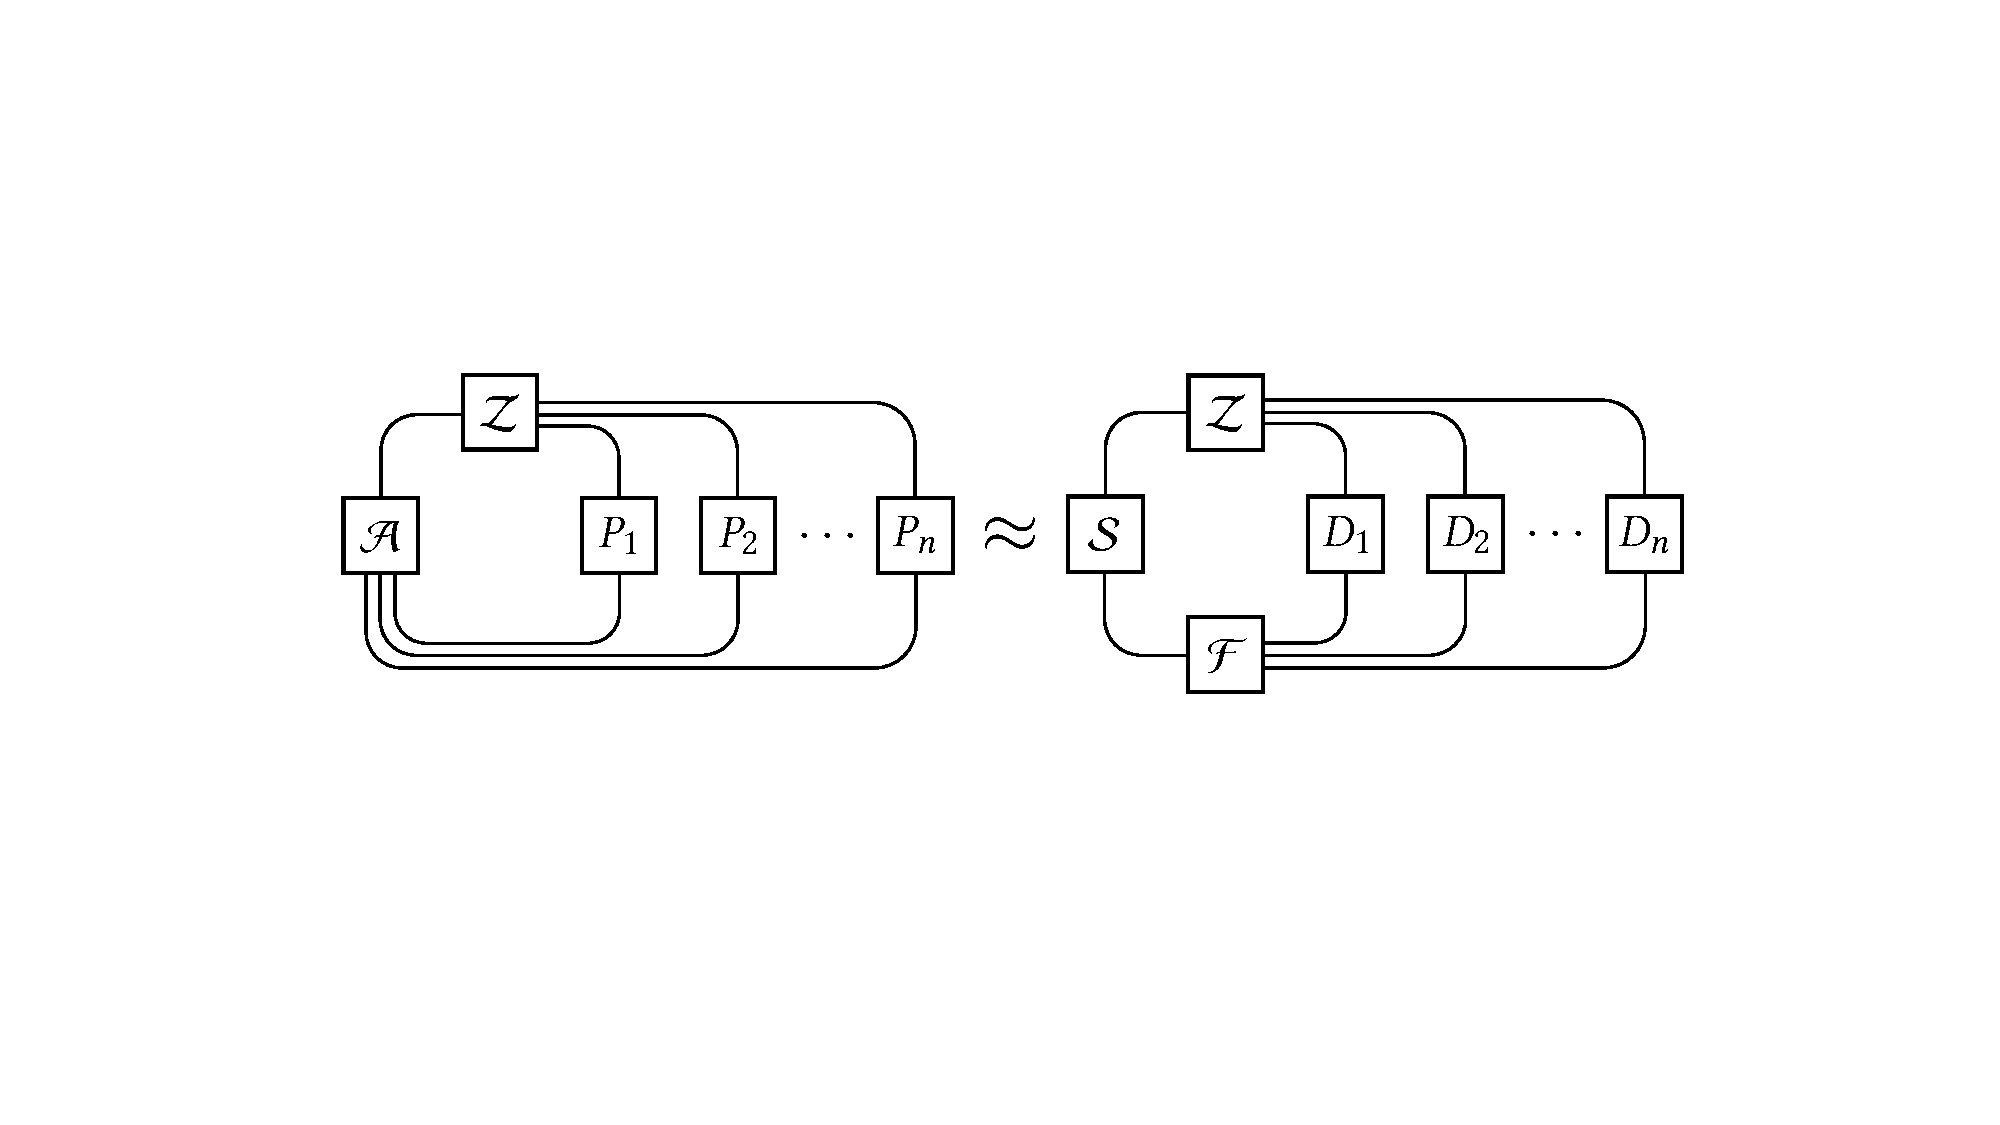
\includegraphics[width=\linewidth]{graphics/uc-experiment}
  \caption{UC experiment with real world (left) and ideal world (right).}
  \label{fig:uc-experiment}
\end{figure}

\begin{figure}
  \centering
  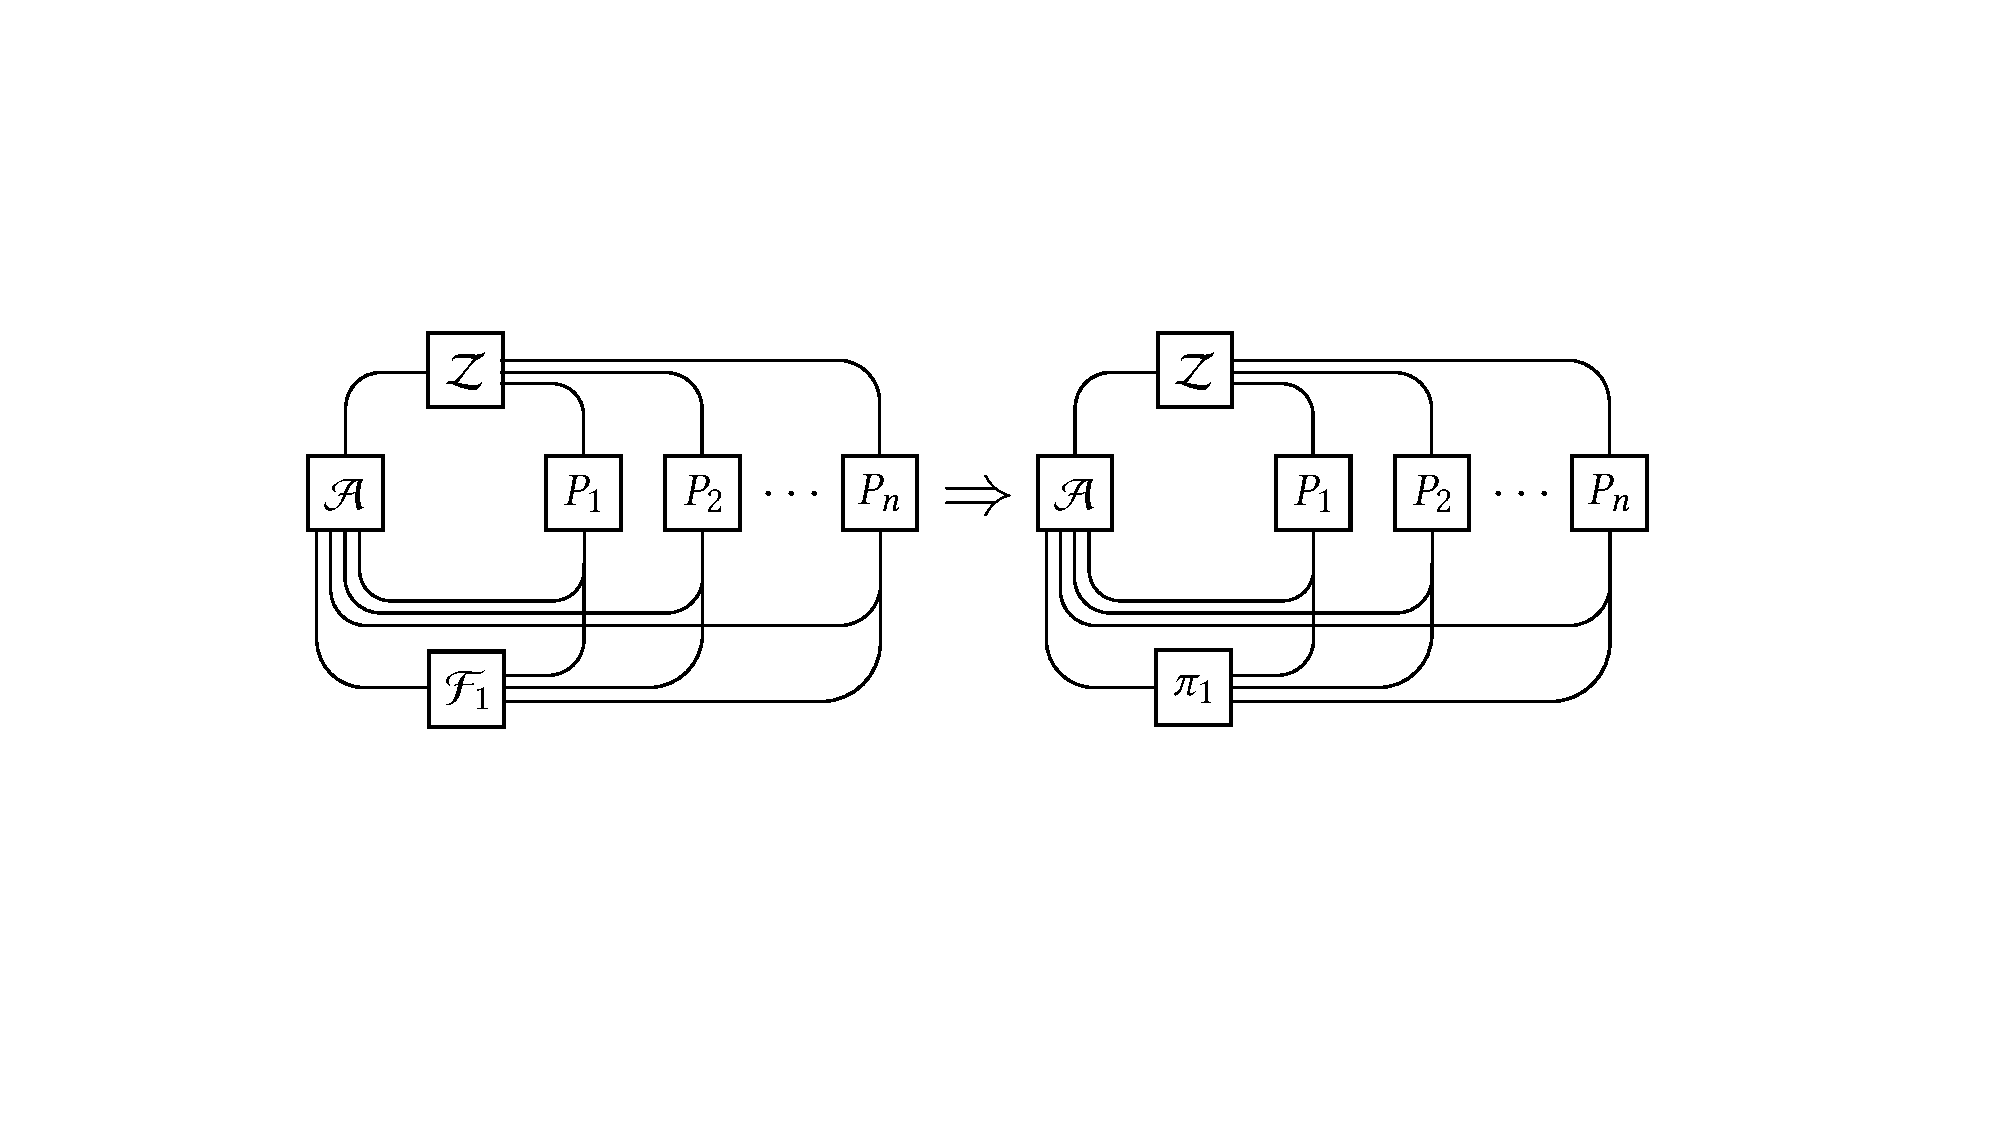
\includegraphics[width=\linewidth]{graphics/composition}
  \caption{UC protocol composition theorem.}
  \label{fig:uc-composition}
\end{figure}
